\documentclass[12pt]{article}
\usepackage[utf8]{inputenc}
\usepackage[T1]{fontenc}
\usepackage[a4paper,left=2cm,right=2cm,top=2cm,bottom=2cm]{geometry}
\usepackage[frenchb]{babel}
\usepackage{libertine}
\usepackage[pdftex]{graphicx}

\setlength{\parindent}{0cm}
\setlength{\parskip}{1ex plus 0.5ex minus 0.2ex}
\newcommand{\hsp}{\hspace{20pt}}
\newcommand{\HRule}{\rule{\linewidth}{0.5mm}}
\def\tab{$\>\>\>\>$}

% insérer une image en fixant la largeur = 0.5 * largeur du document pdf
\newcommand\img[2]{
\begin{figure}[!h]
  \centering
    \includegraphics[width=0.5\paperwidth]{#1}
  \caption{#2}
  \label{img:#1}
\end{figure}
}
%il faut l'utiliser comme ça : \img{image.extension}{légende}
%Pour la citer, utilier \ref{img:image.extension}

\begin{document}

\begin{titlepage}
  \begin{sffamily}
  \begin{center}

    % Upper part of the page. The '~' is needed because \\
    % only works if a paragraph has started.
    
\includegraphics[scale=0.2]{Images/Sorbonne_U.png}~\\[1cm] % mettre le logo de Sorbonne U à la place

    %\textsc{\LARGE Sorbonne Université}\\[1cm]

    \textsc{\Large Licence d'informatique}\\[1.5cm]

    % Title
    \HRule \\[1cm]
    { \huge \bfseries Projet Robotique\\[0.4cm] }

    \HRule \\[1cm]
    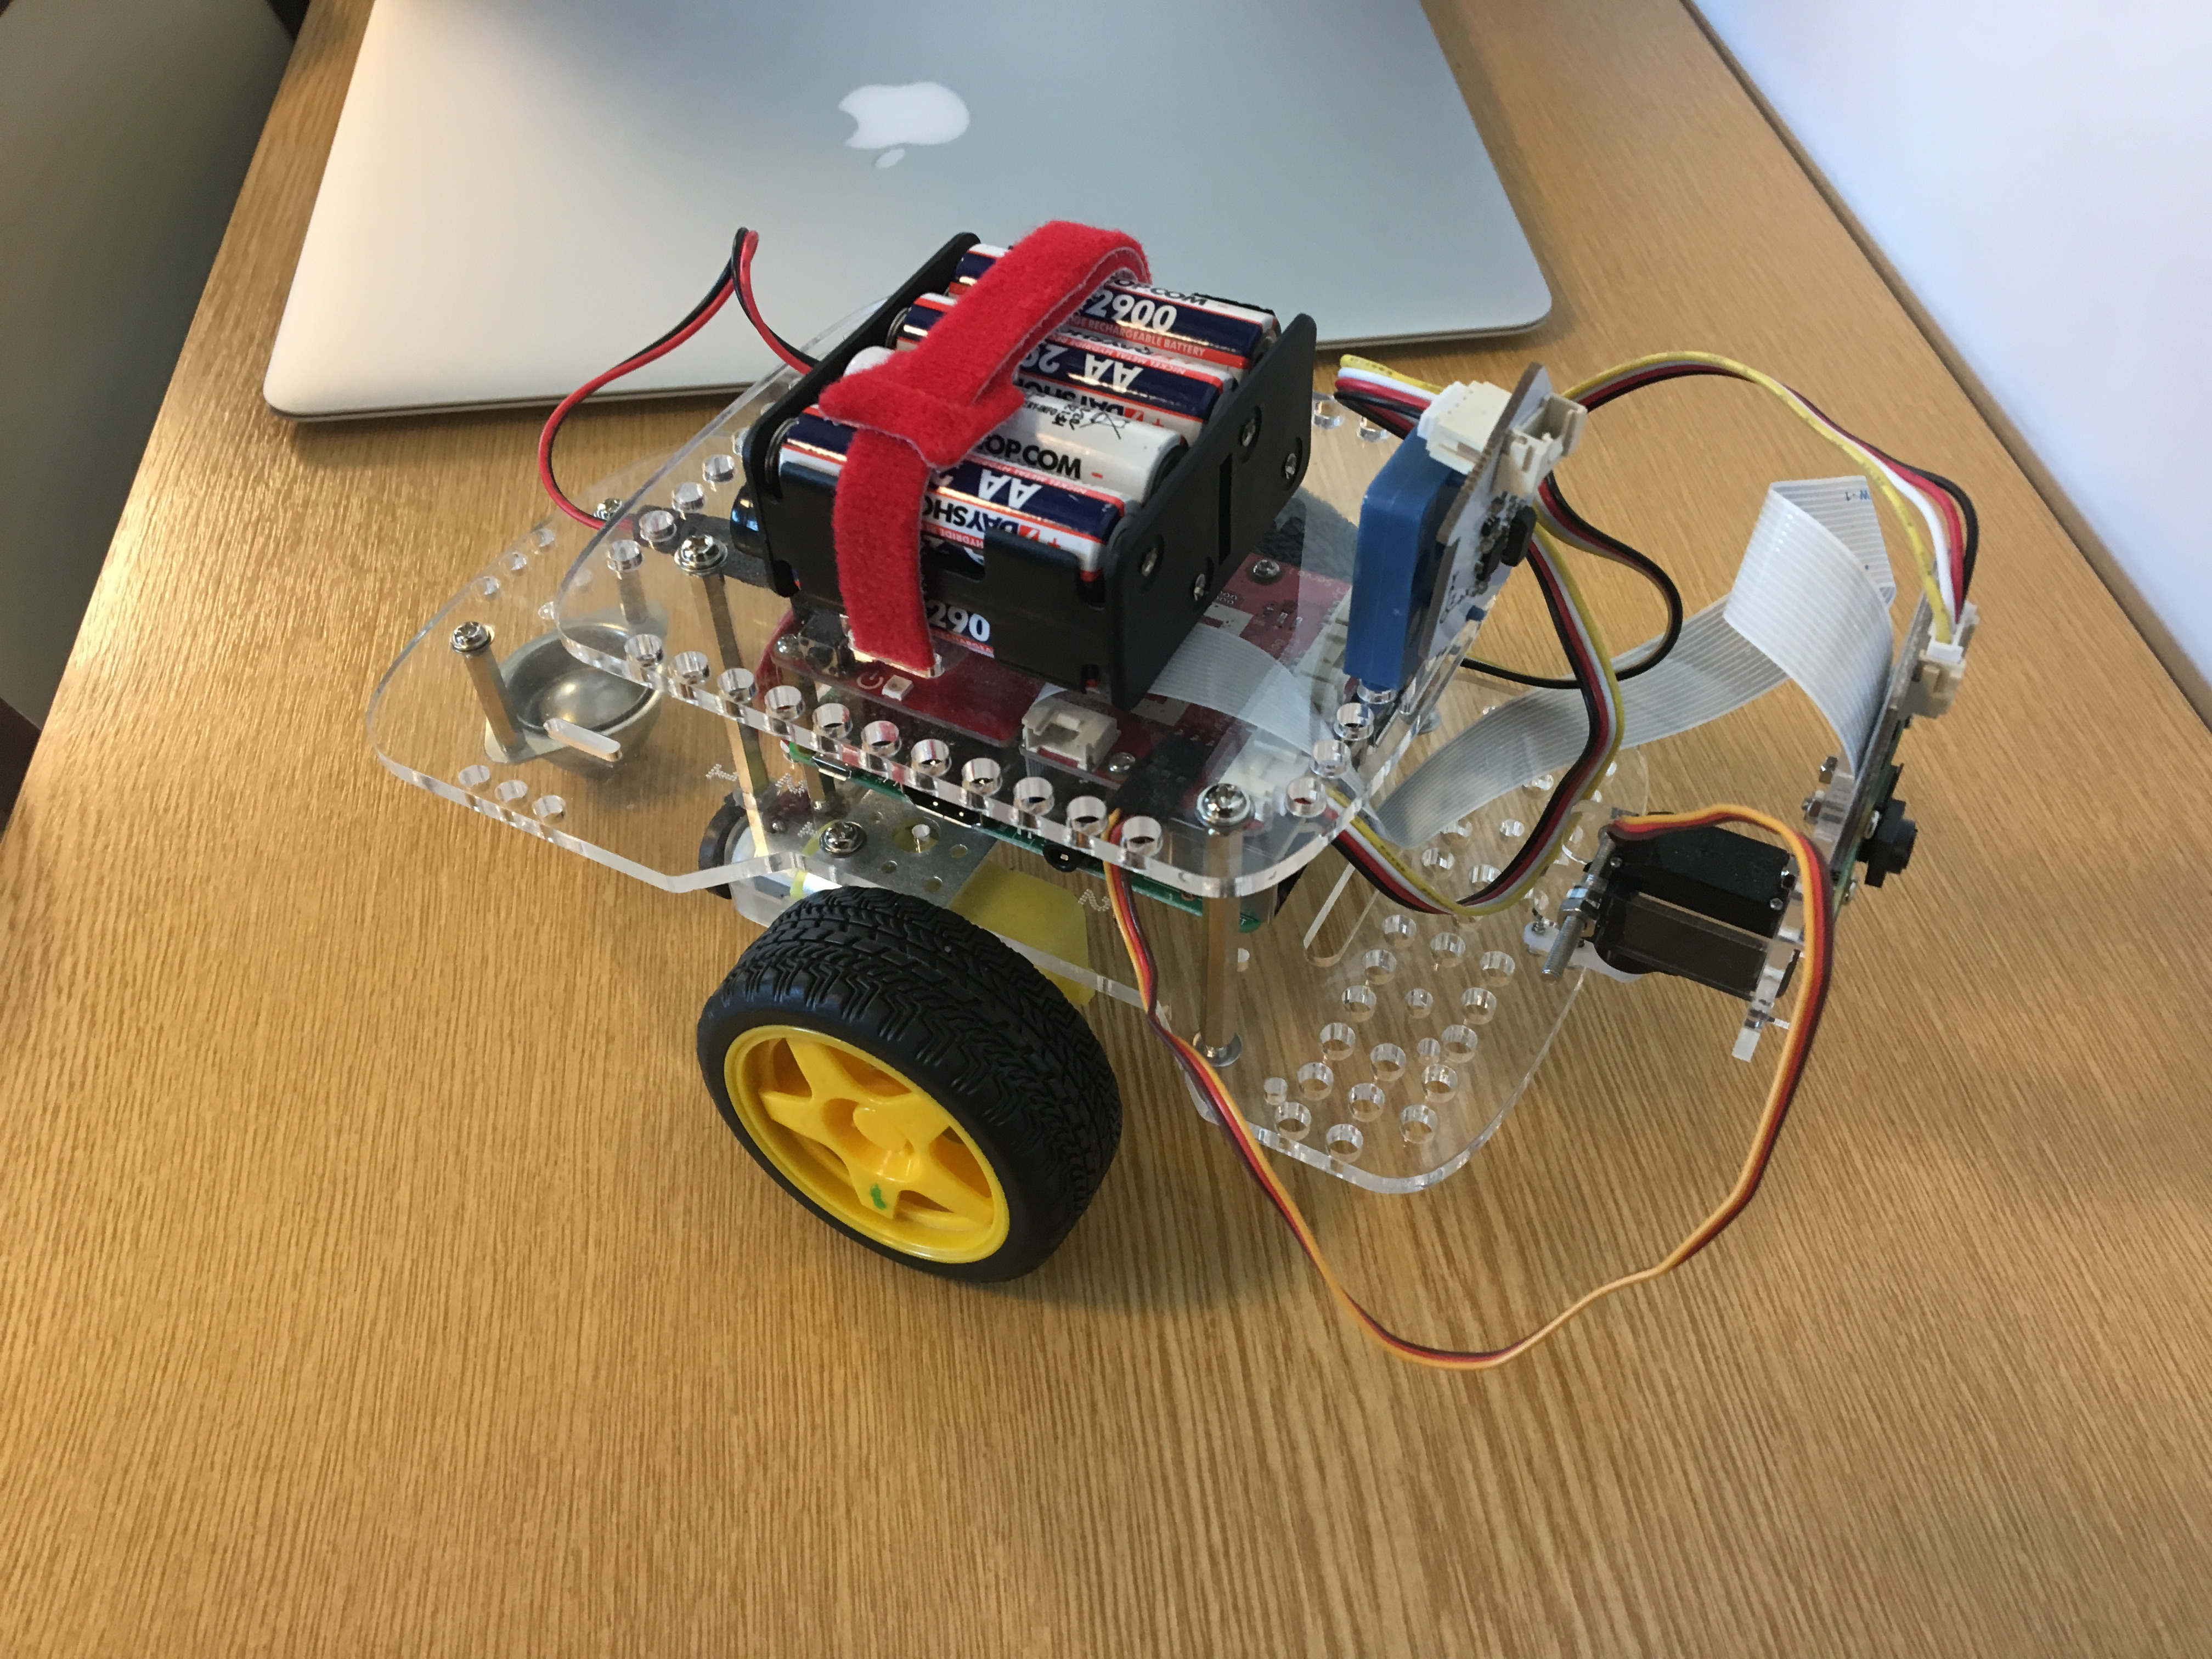
\includegraphics[scale=0.1]{Images/IMG_8579.JPG}
    \\[2cm]

    % Author and supervisor
    \begin{minipage}{0.4\textwidth}
      \begin{flushleft} \large
        Groupe \textsc{FiveGuys}\\
        UE 2I013\\
      \end{flushleft}
    \end{minipage}
    \begin{minipage}{0.4\textwidth}
      \begin{flushright} \large
        \emph{Chargé de cours:} M. \textsc{Baskiotis}\\
        \emph{Chargé de TME:} M. \textsc{Veniat}
      \end{flushright}
    \end{minipage}

    \vfill

    % Bottom of the page
    {\large 1\ier{} Février 2019 — Mai 2019}

  \end{center}
  \end{sffamily}
\end{titlepage}

\tableofcontents
\newpage

\section{Introduction}

\tab Dans le cadre de l'UE 2I013, notre projet était de concevoir un logiciel permettant de contrôler un robot ainsi que son simulateur. Nous avions en charge la totalité du projet et aucun code ne nous était fourni. Nos encadrants étaient à la fois nos superviseurs et nos clients. Il s'agissait donc d'échanger avec eux au sujet des éléments à changer et de l'avancement de notre projet.\\

\tab Les deux objectifs principaux de ce travail étaient : \begin{itemize}
\item[-] la découverte d'un projet de robotique
\item[-] la découverte des méthodes de travail en équipe
\item[]
\end{itemize}

\tab Le projet s'est développé en trois grandes étapes :\begin{itemize}
\item[-] dans un premier temps, il a fallu mettre en place les outils et méthodes nécessaires à notre travail d'équipe
\item[-] dans un deuxième temps, nous avons mis en place les briques de bases de notre projet tel que notre modèle physique ou notre simulateur 2D.
\item[-] pour finir, nous avons commencé à développer les stratégies qui nous permettent de répondre au challenges qui nous on été soumis.
\end{itemize}


\newpage
\section{Rapport}
\subsection{Méthodes et outils}
\subsubsection{Agile/Scrum}

\tab Notre travail ne s'inscrivait pas seulement dans le cadre d'un projet de robotique, il avait également pour but de nous faire découvrir les méthodes de développement en équipe.

\tab En effet, dans les projets que nous réalisions jusqu'alors nous ne nous occcupions pas particulièrement de la façon dont nous allions gérer le développement de nos projets. Les codes à développer sur quelques semaines seulement, en binôme ou trinome, étaient relativement courts et guidés. Dans la plupart des cas, nous avions eu à réaliser des projets pour obtenir directement notre rendu final avec une méthode dite "en V". Cette dernière consiste en un développement du projet de A à Z à partir des exigences du "cahier des charges" (sujet) afin d'obtenir notre application. Les "retours client" se font donc en fin du développement. Il n'y a par conséquent aucune adaptation aux nouvelles exigences du client en cours de projet et les modifications à la fin de celui-ci sont rendues compliquées. Dans nos anciens projets cela ne posait pas problème mais dans le cadre de ce projet oui.

\tab Ce projet était construit de manière à ce que nous développions la totalité du code sur tout le semestre. Il nous fallait donc pouvoir avoir un retour régulier sur l'avancement afin de pouvoir modifier ce qui ne va pas dans la bonne direction et pouvoir s'adapter aux nouvelles exigences pour celui-ci. Nous avons donc chercher à appliquer une autre méthode qui nous a été présentée en cours, la méthode "Agile/Scrum".

\img{Images/VueGlobaleScrum.png}{Schéma méthode Agile/Scrum}

\tab Nous avions donc pour objectif de mettre en place chaque semaine un ensemble de taches les plus petites et indépendantes possible les unes des autres nommées sprint. Les taches devaient toutes être définis avec un maximum de précisions et en concertation avec toute l'équipe pour qu'il n'y ai pas de différence de résultat en fonction du membre du groupe qui l'accompli. Elles ont toutes pour but de remplir un objectif de démonstration concrète de l'avancement du projet au client en terme de nouvelles fonctionnalités. L'objectif final de cette méthode était que chacun des membres du groupe puisse choisir les taches qu'il souhaite accomplir durant la semaine et qui seraient ensuite validées par un autre membre.

\tab A l'issue de la semaine, nous présentions une nouvelle démonstration au client pour obtenir ses retours. Grace aux retours client et au compte-rendu d'équipe rédiger dans la smeiane nous pouvions mettre en place le sprint de la semaine à venir.

\newpage

\subsubsection{Outils pour le travail d'équipe}
\paragraph{Git \& GitHub\\}
\tab Pour pouvoir travailler de façon optimale et sécurisé ils nous fallait pouvoir développer sur un même code sans avoir à se le partager à chaque modifications. Nous avons donc utiliser le logiciel de gestion de version Git afin de conserver une version commune du code la plus à jour afin que chacun puisse travailler dessus à tout moment. La centrasation du code nous permet d'éviter un maximum de les conflits lors du développement du code et de conserver les versions précédentes du code au cas où nous aurions besoin de revenir sur une modification que nous avons apportées au projet et que posent problèmes.

\paragraph{Trello\\}
\tab Pour mettre en place les différentes taches du sprint de la semaine nous avons utiliser le logiciel Trello. Celui-ci nous a permi de rédiger nos cartes pour les différentes taches que nous avions dans notre sprint. Dans un prmier temps l'élaboration de nos sprints et la préparation de nos cartes n'étaient pas très au point ce qui nous conduisait à faire du travail en double où à une mauvaise compréhesion du résultat attendu.

\tab Par la suite, grace aux premières réunions et aux premiers retours, nous avons pu améliorer la préparations de nos sprints. Nous avons donc pu avancer dans la préparation de notre simulateur avec une première interface et la mise en place de notre modèle.
%\paragraph{Slack \& Whatsapp\\}

%\paragraph{Python\\}

\subsubsection{Hiérarchie du code}

\paragraph{MVC (Model-View-Controler)\\}

\paragraph{Hiérarchie de notre code\\}

\begin{center}
Juste un schéma ?
\end{center}

\newpage
\subsection{Mise en place de briques de base}
\subsubsection{Modélisation du réel}
\tab Comme nous le savons, le but du projet est de modéliser les différents comportements d’un robot dans son environnement. Autrement dit, le déplacement d’un robot dans une arène semée d’obstacles. Nous remarquons ainsi la présence des termes de nos objets de bases : une arène, un robot et des obstacles.
\paragraph{Notre Arène\\}
Le terme d’arène peut être vulgarisé par le terme d’espace. C’est l’environnement dans lequel nous allons conserver nos données. Quoi de mieux qu’une matrice ? Une matrice MxN est un tableau de nombres à M lignes et N colonnes. Les nombres présents dans la matrice sont appelés « éléments de la matrice ».  Ce type de tableau va nous permettre de différencier les objets présents ainsi que leurs coordonnées. Par exemple, nous avons de décidé d’attribuer le chiffre, « 0 » aux emplacements vides, « 1 » au centre de notre robot et « 2 » aux zones occupées par des obstacles. Pour résumer, grâce à cette perspective nous pouvons savoir où se trouve notre robot et si un objet est présent à la colonne x et à la ligne y.
\paragraph{Notre Robot\\}
Nous avons décidé de modéliser notre robot comme un rectangle muni d’un angle de direction car ce sont les concepts de base se rapprochant au maximum de nos contraintes dans notre contexte. Son corps est ainsi un rectangle (rouge) muni d’une certaine longueur et d’une certaine largeur. Si nous voulons savoir où se trouve notre robot, nous avons qu’à parcourir la matrice et chercher l’élément ayant pour valeur « 1 ». Cependant, cela ne correspond qu’au centre du robot et non l’espace total qu’il occupe. Nous savons que notre robot possède un centre de coordonnées [ x , y ], une longueur et une largeur. Ainsi, l’espace occupé est réellement tous les éléments de l’arène ayant une abscisse comprise entre ‘ ’x – largeur /2 ’’ et ‘’x + largeur/2’’ et une ordonnée comprise entre ‘ ’y – longueur /2 ’’ et ‘’y + longueur/2’’. Pour mieux visualiser, vous trouverez un schéma ci-dessous :

\paragraph{Nos Obstacles\\}
Dans la même idée que pour notre robot, nos obstacles sont modélisés par des rectangles noirs, avec une longueur et une largeur. Dans notre matrice, leur centre correspondent aux éléments « 2 ». Les différencier par la valeur de leurs éléments va nous permettre de connaître, par exemple, leur nombre, leurs coordonnées et l’espace qu’ils occupent individuellement. Cela va nous être très utile pour transmettre à notre robot quelles zones il doit contourner.

\subsubsection{Mise en place de l'interface graphique 2D}

\subsubsection{Stratégies de base}
\paragraph{Ligne droite\\}
Notre premier objectif a été de faire avancer notre robot en ligne droite. Pour cela, nous réalisions une modification des coordonnées du robot pour le déplacer d'une distance fournie en argument. Pour le faire avancer en ligne droite selon son orientation, nous avons au robot un paramètre d'angle qui indique à tout moment son orientation sur le cercle trigonométrique. Ainsi, les fonctions trigonométriques nous permettaient de facilement coefficienter la modification des paramètres, et donc de le faire se déplacer dans la bonne direction.

\paragraph{Rotation\\}
Le second objectif a été de déterminer comment faire tourner le robot. La méthode la plus simple était de le faire tourner sur lui-même, n'ayant pas à gérer de modification de ses coordonnées. L'implémentation du paramètre d'angle a grandement facilité la réalisation de cette fonction, puisque réduite a une modification de paramètre.

\paragraph{Detection d'obstacles\\}
Le robot étant doté d'un capteur permettant de déterminer sa distance à un obstacle devant lui, il nous fallait inclure cette fonctionnalité à notre robot simulé. Pour cela nous avons implémenté un capteur, qui au lancement de la fonction se déplace en ligne droite en partant du robot d'un pas fourni en argument, et selon la même procédure de calcul que pour de déplacement du robot. A chaque pas, le capteur observe la valeur de la matrice sur ses coordonées. S'il détecte un "0", il continue à avancer, s'il rencontre un "2" (un obstacle), il s'arrête et la fonction renvoie les dernières coordonnées du capteur, qui étaient ensuite interprétées pour calculer la distance à l'obstacle.

\subsubsection{Passage de la simulation au réel}
\tab L'une des exigences pour projet était que notre code ne devais pas dépendre du fait que celui-ci soit lancé dans notre simulateur ou dans notre robot. Le but étant de pouvoir tester les nouvelles fonctionnalitées de notre robot nous voulions ajouter comme si elle était déjà dans le robot. Ainsi l'implémentation dans le robot peut être direct et normalement sans bug. Les seules corrections que

\newpage
\subsection{Développement des stratégies}
\subsubsection{Stratégie carré}
\subsubsection{Stratégie détection de mur}
\subsubsection{Stratégie cercle}
\subsubsection{Stratégie contourner une porte}
\subsubsection{Stratégie détection balise}

\newpage

\section{Remerciements}

\newpage

\section{Conclusion}
\end{document}
